\documentclass[border=0,tikz]{standalone}
\usepackage{amsmath}
\usepackage{physics}
\usepackage{times}
\usetikzlibrary{intersections}
\usetikzlibrary{calc}
\usetikzlibrary{patterns}

% TikZ styles
\definecolor{blue}{rgb}{0.035, 0.471, 0.671}
\definecolor{red}{rgb}{0.5,0,0}
\tikzstyle{vsia}=[blue, thick]
\tikzstyle{vssa}=[red, thick]

% notations
\newcommand{\vect}[1]{\va*{#1}} % bold arrow vectors
\newcommand{\vv}[0]{\vect{v}}           % velocity vector
\newcommand{\vsia}[0]{\vv_{\mathrm{SIA}}}   % SIA velocity
\newcommand{\vssa}[0]{\vv_{\mathrm{SSA}}}   % SSA velocity

% begin document
\begin{document}
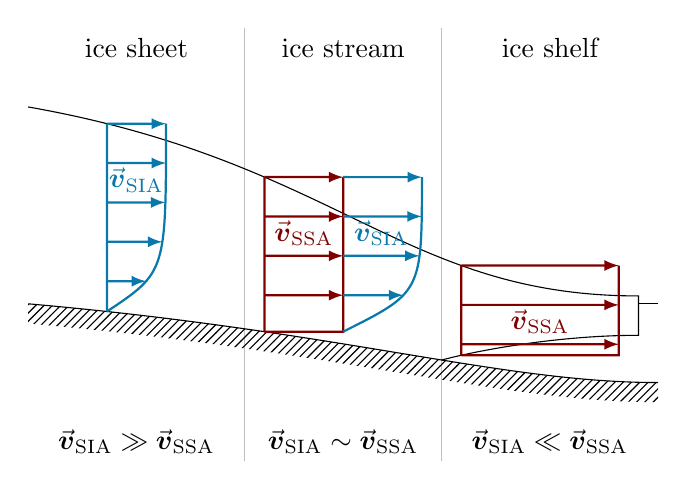
\begin{tikzpicture}[>=latex]

% white background
\fill[white] (0,0) rectangle +(8.0,5.5);
%\draw [help lines, lightgray] (0,0) grid (8.0,5.5);

% transition lines and calving front coordinates
\coordinate (tr1) at (2.75, 0);  % transition one
\coordinate (tr2) at (5.25, 0);  % transition two
\coordinate (cf) at (7.75, 2);
\draw[lightgray, name path=tr1] (tr1 |- 0,0) -- +(0,5.5) ;
\draw[lightgray, name path=tr2] (tr2 |- 0,0) -- +(0,5.5) ;

% location of the velocity profiles
\path [name path=x1] (1.0,0) -- +(0,5) ;
\path [name path=x2] (3.0,0) -- +(0,5) ;
\path [name path=x3] (5.5,0) -- +(0,5) ;

% bedrock topography
\draw [name path=bed]
    (0,2) .. controls +(-5:4) and +(180:2) .. (8,1);
\fill [pattern=north east lines]
    (0,2) .. controls +(-5:4) and +(180:2) .. (8,1)
          -- +(0,-0.25)
          .. controls +(180:2) and +(-5:4) .. (0,1.75);

% locate the grounding line
\path [name intersections={of=bed and tr2, by=gl}] ;

% surface topograpy
\draw [name path=surf]
    (0,4.5) .. controls +(-10:4) and +(180:3) .. ($(cf)+(0,0.1)$)
          -- (cf) ;

% ice shelf base
\draw [name path=base]
    (gl) .. controls +(15:0.5) and +(180:1) .. ($(cf)-(0,0.4)$)
         -- (cf);

% sea level
\draw [name path=sl] (cf) -- (cf -| 8,0) ;

% first velocity profile
\path [name intersections={of=surf and x1, by=s1}] ;
\path [name intersections={of=bed and x1, by=b1}] ;
\draw[vsia] (b1) -- (s1);
\draw[vsia, name path=vsia]
    (b1) .. controls ++(0.75,0.5) .. ($(s1)+(0.75,0)$);

% first velocity vectors
\path[name path=vgrid] (s1) foreach \x in {1,...,5} { -- +(2,0) ++(0,-0.5) };
\path[name intersections={of=x1 and vgrid, name=a, total=\t}];
\path[name intersections={of=vsia and vgrid, name=b, total=\t}];
\draw[vsia, ->] (a-1) -- (b-1);
\draw[vsia, ->] (a-2) -- (b-2);
\draw[vsia, ->] (a-3) -- (b-3) node [midway, above] {$\vsia$};
\draw[vsia, ->] (a-4) -- (b-4);
\draw[vsia, ->] (a-5) -- (b-5);

% second velocity profile
\path [name intersections={of=surf and x2, by=s2}] ;
\path [name intersections={of=bed and x2, by=b2}] ;
\draw[vssa] (b2) -- (s2);
\draw[vssa, name path=vssa]
    (b2) -- ($(b2)+(1,0)$) -- ($(s2)+(1,0)$);
\draw[vsia, name path=vsia]
    ($(b2)+(1,0)$) .. controls ++(1,0.5) .. ($(s2)+(2,0)$);

% second velocity vectors
\path[name path=vgrid] (s2) foreach \x in {1,...,5} { -- +(2,0) ++(0,-0.5) };
\path[name intersections={of=x2 and vgrid, name=a, total=\t}];
\path[name intersections={of=vssa and vgrid, name=b, total=\t}];
\path[name intersections={of=vsia and vgrid, name=c, total=\t}];
\draw[vssa, ->] (a-1) -- (b-1);
\draw[vssa, ->] (a-2) -- (b-2);
\draw[vssa, ->] (a-3) -- (b-3) node [midway, above] {$\vssa$};
\draw[vssa, ->] (a-4) -- (b-4);
\draw[vsia, ->] (b-1) -- (c-1);
\draw[vsia, ->] (b-2) -- (c-2);
\draw[vsia, ->] (b-3) -- (c-3) node [midway, above] {$\vsia$};
\draw[vsia, ->] (b-4) -- (c-4);

% third velocity profile
\path [name intersections={of=surf and x3, by=s3}] ;
\path [name intersections={of=base and x3, by=b3}] ;
\draw[vssa] (b3) -- (s3);
\draw[vssa, name path=vssa]
    (b3) -- ($(b3)+(2,0)$) -- ($(s3)+(2,0)$);

% third velocity vectors
\path[name path=vgrid] (s3) foreach \x in {1,...,3} { -- +(2,0) ++(0,-0.5) };
\path[name intersections={of=x3 and vgrid, name=a, total=\t}];
\path[name intersections={of=vssa and vgrid, name=b, total=\t}];
\draw[vssa, ->] (a-1) -- (b-1);
\draw[vssa, ->] (a-2) -- (b-2);
\draw[vssa, ->] (a-3) -- (b-3) node [midway, above] {$\vssa$};

% add transition lines and annotations
\coordinate (m1) at ($(0,0)!0.5!(tr1)$) ;
\coordinate (m2) at ($(tr1)!0.5!(gl)$) ;
\coordinate (m3) at ($(gl)!0.5!(8,0)$) ;
\coordinate (top) at ($(0,5.25)$) ;
\coordinate (bot) at ($(0,0.25)$) ;

\node at (m1|-top) {ice sheet};
\node at (m2|-top) {ice stream};
\node at (m3|-top) {ice shelf};
\node at (m1|-bot) {$\vsia\gg\vssa$};
\node at (m2|-bot) {$\vsia\sim\vssa$};
\node at (m3|-bot) {$\vsia\ll\vssa$};

\end{tikzpicture}
\end{document}
